\documentclass{article}
\usepackage{tikz}
\usetikzlibrary{arrows.meta, positioning, shapes.geometric}
\usepackage[utf8]{inputenc}
\usepackage[UTF8]{ctex}
% \setCJKmainfont{}
\usepackage{amsmath}
\usepackage{amssymb}
\usepackage{array}
\usepackage{booktabs}
\usepackage{enumitem}
\usepackage{xeCJK}
\usepackage{CJKutf8}
\setCJKmainfont{Noto Serif CJK TC}    % 思源宋體繁體版(推薦)
\setCJKsansfont{Microsoft JhengHei}   % 微軟正黑體
\setCJKmonofont{Noto Sans Mono CJK TC}
% \setCJKmainfont{WenQuanYi Zen Hei}
% % 或者使用其他可用字體:
% % \setCJKmainfont{AR PL Mingti2L Big5}
% % \setCJKmainfont{Noto Sans CJK TC}

% % 設置全形符號支持
% \setCJKsansfont{WenQuanYi Zen Hei}
% \setCJKmonofont{WenQuanYi Zen Hei}

\title{Self-Injection-Locked (SIL) Oscillator Analysis}
\author{carlos ma}
\date{\today}

\begin{document}
\maketitle

\section{General Definition}

\textbf{Resonance} occurs when a system is subjected to an external force or signal whose frequency matches the system's \textbf{natural frequency}, resulting in a large increase in amplitude.

\section{Real-World Examples}

\begin{center}
\begin{tabular}{>{\centering\arraybackslash}m{3cm} >{\raggedright\arraybackslash}m{9cm}}
\toprule
\textbf{Context} & \textbf{Description} \\
\midrule
Violin string & Vibrates strongly when bowing matches its natural vibration frequency \\
RF circuits & LC circuits resonate at a specific frequency $\rightarrow$ used in filters, radios \\
Bridges & Tacoma Narrows Bridge collapsed due to wind-induced resonance \\
SIL radar & Resonator oscillates strongly at $\omega_n$; injection close to $\omega_n$ causes locking \\
\bottomrule
\end{tabular}
\end{center}

\section{In Engineering Terms}

For a \textbf{second-order system} like an RLC circuit or mechanical spring-mass-damper system:

\subsection{Natural Frequency}
\begin{align}
\omega_n &= \sqrt{\frac{k}{m}} \quad \text{(mechanical)} \\
\omega_n &= \frac{1}{\sqrt{LC}} \quad \text{(electrical)}
\end{align}

When driven at $\omega = \omega_n$, the system exhibits \textbf{maximum energy transfer} and large amplitude.

\section{Resonance Graphically}

If you plot amplitude vs frequency, the \textbf{resonance peak} appears at $\omega_n$, especially if the system has \textbf{high quality factor (Q)}.

\section{In Self-Injection Locked Oscillators}

In SIL systems:
\begin{itemize}
    \item The oscillator has a \textbf{resonant frequency} $\omega_n$
    \item The feedback (injection) signal, when close to $\omega_n$, causes the oscillator to \textbf{lock its frequency and phase}
    \item This locking happens more efficiently \textbf{because of resonance}
\end{itemize}

\section{Summary}

\begin{center}
\begin{tabular}{>{\centering\arraybackslash}m{4cm} >{\raggedright\arraybackslash}m{8cm}}
\toprule
\textbf{Term} & \textbf{Meaning} \\
\midrule
Resonance & Strong response when input $\approx$ natural frequency \\
Natural Frequency & The frequency a system ``prefers'' to oscillate at \\
Quality Factor (Q) & Determines how sharp/narrow the resonance is \\
\bottomrule
\end{tabular}
\end{center}

\section{Adler's Equation (Simplified Form)}
    
\begin{equation}
\frac{d\phi(t)}{dt} = \Delta \omega - K \cdot \sin(\phi(t))
\end{equation}

Where:
\begin{itemize}
    \item $\phi(t)$: phase difference between oscillator and injection signal
    \item $\Delta \omega = \omega_{\text{inj}} - \omega_0$: natural frequency difference
    \item $K$: coupling strength (determined by injection energy and oscillator Q factor)
\end{itemize}

\section{Notes for SIL Radar}

Excellent question! That equation:

\begin{equation}
\omega(t) - \omega_n \approx -\frac{\omega_n}{2Q} \cdot \frac{B}{A} \cdot \sin[\theta(t)]
\end{equation}

comes from analyzing \textbf{self-injection-locked (SIL)} oscillators --- specifically how \textbf{injection} of a reflected signal modifies the \textbf{oscillator's instantaneous frequency}.

Let me explain \textbf{step by step} how this equation is derived from the physics of a resonator-based oscillator subject to weak injection:

\subsection{Context}

\begin{itemize}
    \item $\omega_n$: natural frequency of the oscillator (free-running)
    \item $\omega(t)$: actual instantaneous frequency when injection is present
    \item $Q$: quality factor of the oscillator (higher $\rightarrow$ sharper resonance)
    \item $A$: amplitude of the oscillator signal
    \item $B$: amplitude of the injected signal (typically a reflected echo)
    \item $\theta(t)$: phase difference between injected and oscillator signals
\end{itemize}

\subsection{Step-by-step Derivation}

\subsubsection{Step 1: Start from the complex oscillator dynamics}

In oscillator theory, a sinusoidal oscillator's dynamics near resonance can be described using \textbf{complex envelope} notation:

Let the oscillator's complex amplitude be:
\begin{equation}
z(t) = A(t) e^{j\phi(t)}
\end{equation}

Assuming a self-sustained oscillator with \textbf{external injection} $B e^{j(\omega_{\text{inj}} t + \phi_B)}$, its dynamics can be modeled using a \textbf{resonator differential equation}:

\begin{equation}
\frac{dz}{dt} + \left(j\omega_n + \frac{\omega_n}{2Q}\right) z = \frac{\omega_n}{2Q} B e^{j(\omega_{\text{inj}} t + \phi_B)}
\end{equation}

Here:
\begin{itemize}
    \item The term on the left is the oscillator's natural decay and oscillation
    \item The term on the right is \textbf{external drive (injection)}
\end{itemize}

\subsubsection{Step 2: Assume steady-state, decompose phase dynamics}

Let:
\begin{itemize}
    \item $z(t) = A e^{j\omega(t)t}$
    \item Assume \textbf{injection frequency is close to $\omega_n$} $\rightarrow$ do slow-varying approximation
    \item Define $\theta(t) = \phi(t) - \omega_{\text{inj}} t$ as the phase difference between oscillator and injected signal
\end{itemize}

Then, you can extract the \textbf{phase evolution}:
\begin{equation}
\frac{d\theta}{dt} = \omega(t) - \omega_{\text{inj}} \approx \omega(t) - \omega_n
\end{equation}

That's the \textbf{phase error rate}.

\subsubsection{Step 3: Linearize injection-locking force}

From resonator theory (and RF oscillator models), the effect of injection is to ``pull'' the oscillator frequency, and that pulling is \textbf{proportional to the sine of the phase difference} $\sin(\theta)$.

From the forced oscillator dynamics and projection onto quadrature component, we get:
\begin{equation}
\omega(t) - \omega_n \approx -\frac{\omega_n}{2Q} \cdot \frac{B}{A} \cdot \sin[\theta(t)]
\end{equation}

This is the approximate \textbf{Adler-type equation} specifically for a SIL system using a resonator.

\subsection{Physical Meaning}

\begin{center}
\begin{tabular}{>{\centering\arraybackslash}m{3cm} >{\raggedright\arraybackslash}m{8cm}}
\toprule
\textbf{Term} & \textbf{Meaning} \\
\midrule
$\omega(t) - \omega_n$ & How much the oscillator's frequency is ``pulled'' \\
$\frac{\omega_n}{2Q}$ & Sets the \textbf{natural bandwidth} of the oscillator's response \\
$\frac{B}{A}$ & Strength of the injected signal relative to self-oscillation amplitude \\
$\sin(\theta(t))$ & Phase interaction term driving the frequency shift \\
\bottomrule
\end{tabular}
\end{center}

\section{Explain Adler Equation with Block Diagram}

This equation comes from:
\begin{enumerate}
    \item Resonator + injection modeling
    \item Linearized oscillator dynamics near steady-state
    \item Projection of injection onto oscillator's quadrature axis
    \item Assuming small amplitude variation (constant envelope)
\end{enumerate}

It is \textbf{more specific than Adler's equation}, applying directly to SIL oscillators with $Q$-limited resonators.

\subsection{Adler Equation Block Diagram}

% \begin{center}
    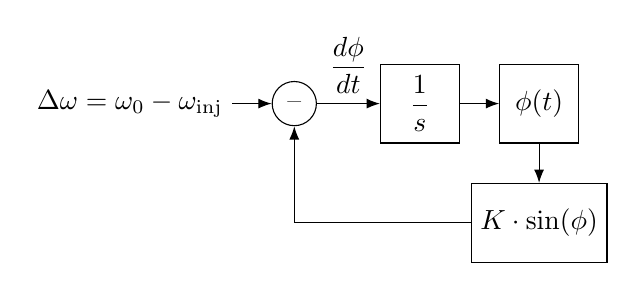
\begin{tikzpicture}[auto, node distance=2.5cm, >=Latex]

        % Nodes
        \node[left] (delta) {\( \Delta\omega = \omega_0 - \omega_{\text{inj}} \)};
        \node[draw, circle, minimum size=0/3cm, right=0.5cm of delta] (sum) {--};
        \node[draw, rectangle, minimum width=1cm, minimum height=1cm, right=0.8cm of sum] (int) {\( \dfrac{1}{s} \)};
        \node[draw, rectangle, minimum width=1cm, minimum height=1cm, right=0.5cm of int] (phi) {\( \phi(t) \)};
        \node[draw, rectangle, minimum width=1cm, minimum height=1cm, below=0.5cm of phi] (sin) {\( K \cdot \sin(\phi) \)};
      
        % Arrows
        \draw[->] (delta) -- (sum);
        \draw[->] (sum) -- node {\( \dfrac{d\phi}{dt} \)} (int);
        \draw[->] (int) -- (phi);
        \draw[->] (phi) -- (sin);
        \draw[->] (sin) -| (sum.south);
      
      \end{tikzpicture}
% \end{center}

The block diagram shows:
\begin{itemize}
    \item \textbf{Input}: Frequency difference $\Delta \omega = \omega_{\text{inj}} - \omega_0$
    \item \textbf{Nonlinear feedback}: $K\sin(\phi)$ represents injection locking force
    \item \textbf{Integrator}: Converts frequency difference to phase
    \item \textbf{Output}: Phase difference $\phi(t)$
\end{itemize}

% \usepackage{amsmath}
% \begin{left}

% \end{left}
\section*{RF信號的IQ表示法}

一個簡單的數學表示:

若原始 RF 信號為:
\[
s(t) = A(t) \cdot \cos\left(2\pi f_c t + \phi(t)\right)
\]

它可以轉換為 IQ 表示為:
\[
s(t) = I(t) \cdot \cos\left(2\pi f_c t\right) - Q(t) \cdot \sin\left(2\pi f_c t\right)
\]

其中:
\[
\begin{aligned}
I(t) &= A(t) \cdot \cos\left(\phi(t)\right) \\
Q(t) &= A(t) \cdot \sin\left(\phi(t)\right)
\end{aligned}
\]

\subsection*{舉例:16-QAM}

例如在 16-QAM(Quadrature Amplitude Modulation)中,每個符號都會有一組對應的 $I$ 和 $Q$ 值,用以決定其在星座圖(constellation diagram)中的位置。

\section{系統分類}

根據開迴路傳遞函數中積分器的個數,將系統分為:

\begin{itemize}
    \item \textbf{0型系統}:無積分器
    \item \textbf{I型系統}:有1個積分器
    \item \textbf{II型系統}:有2個積分器
\end{itemize}

\section{誤差係數與穩態誤差}

\subsection{位移誤差係數 ($K_p$)}

\begin{equation}
K_p = \lim_{s \to 0} G(s)H(s)
\end{equation}

對於單位階躍輸入 $r(t) = 1$:
\begin{itemize}
    \item 0型系統:$e_{ss} = \frac{1}{1+K_p}$
    \item I型和II型系統:$e_{ss} = 0$
\end{itemize}

\subsection{速度誤差係數 ($K_v$)}

\begin{equation}
K_v = \lim_{s \to 0} sG(s)H(s)
\end{equation}

對於單位斜坡輸入 $r(t) = t$:
\begin{itemize}
    \item 0型系統:$e_{ss} = \infty$
    \item I型系統:$e_{ss} = \frac{1}{K_v}$
    \item II型系統:$e_{ss} = 0$
\end{itemize}

\subsection{加速度誤差係數 ($K_a$)}

\begin{equation}
K_a = \lim_{s \to 0} s^2G(s)H(s)
\end{equation}

對於單位拋物線輸入 $r(t) = \frac{t^2}{2}$:
\begin{itemize}
    \item 0型和I型系統:$e_{ss} = \infty$
    \item II型系統:$e_{ss} = \frac{1}{K_a}$
\end{itemize}

\section{實際評估步驟}

\begin{enumerate}
    \item \textbf{確定系統型別}:分析開迴路傳遞函數,計算積分器個數
    \item \textbf{計算誤差係數}:根據系統型別計算相應的$K_p$、$K_v$、$K_a$
    \item \textbf{選擇測試輸入}:使用階躍、斜坡、拋物線輸入
    \item \textbf{計算穩態誤差}:利用最終值定理或誤差係數公式
    \item \textbf{時域仿真驗證}:透過數值仿真觀察實際誤差行為
\end{enumerate}

\section{改善誤差的方法}

\begin{itemize}
    \item 增加系統型別(增加積分器)
    \item 提高開迴路增益
    \item 加入前饋補償
    \item 使用PID控制器
\end{itemize}

這種系統性的分析方法能夠有效預測和改善控制系統的穩態性能。


\section{Starting Point: Simple Harmonic Oscillator}

We begin with the basic oscillator equation:

\begin{equation}
\ddot{x} + \omega_0^2 x = 0
\end{equation}

This represents a \textbf{lossless oscillator} (like a perfect spring-mass system or LC circuit).

\section{Problem: Real Oscillators Have Losses}

In reality, all oscillators lose energy due to:
\begin{itemize}
    \item \textbf{Resistance} (in electrical circuits)
    \item \textbf{Friction} (in mechanical systems)
    \item \textbf{Radiation} (in antennas)
\end{itemize}

So we add a damping term:

\begin{equation}
\ddot{x} + \gamma\dot{x} + \omega_0^2 x = 0
\end{equation}

\textbf{Problem}: This just decays to zero! Real oscillators like \textbf{radio transmitters} or \textbf{clock circuits} need to sustain themselves.

\section{Solution: Add Energy Source}

To maintain oscillation, we need to \textbf{inject energy} into the system. But we want \textbf{smart energy injection} that:
\begin{itemize}
    \item Adds energy when oscillation is small
    \item Removes energy when oscillation gets too large
    \item Results in \textbf{stable amplitude}
\end{itemize}

\section{Van der Pol's Brilliant Insight}

Van der Pol (1920s) proposed \textbf{nonlinear damping}:

\begin{equation}
\ddot{x} - \mu(1 - x^2)\dot{x} + \omega_0^2 x = 0
\end{equation}

Let's analyze the damping term: $-\mu(1 - x^2)\dot{x}$

\subsection{Case 1: Small Oscillations ($|x| \ll 1$)}

When $x$ is small: $x^2 \approx 0$, so:

\begin{equation}
(1 - x^2) \approx 1
\end{equation}

The equation becomes:

\begin{equation}
\ddot{x} - \mu\dot{x} + \omega_0^2 x \approx 0
\end{equation}

\textbf{Negative damping coefficient} ($-\mu$)! This means:
\begin{itemize}
    \item \textbf{Energy is being added} to the system
    \item Small oscillations \textbf{grow exponentially}
\end{itemize}

\subsection{Case 2: Large Oscillations ($|x| \gg 1$)}

When $x$ is large: $x^2 \gg 1$, so:

\begin{equation}
(1 - x^2) \approx -x^2 \quad \text{(negative!)}
\end{equation}

The equation becomes:

\begin{equation}
\ddot{x} - \mu(-x^2)\dot{x} + \omega_0^2 x = \ddot{x} + \mu x^2\dot{x} + \omega_0^2 x \approx 0
\end{equation}

Now we have \textbf{positive damping} ($+\mu x^2$)! This means:
\begin{itemize}
    \item \textbf{Energy is being removed} from the system
    \item Large oscillations are \textbf{suppressed}
\end{itemize}

\section{Physical Interpretation}

\subsection{The Magic Balance}

The Van der Pol oscillator \textbf{automatically regulates its amplitude}:

\begin{enumerate}
    \item \textbf{If amplitude is too small} $\rightarrow$ Negative damping $\rightarrow$ Energy added $\rightarrow$ Amplitude grows
    \item \textbf{If amplitude is too large} $\rightarrow$ Positive damping $\rightarrow$ Energy removed $\rightarrow$ Amplitude shrinks
    \item \textbf{At just the right amplitude} $\rightarrow$ Zero net damping $\rightarrow$ \textbf{Stable limit cycle}
\end{enumerate}

\subsection{Real-World Examples}

\textbf{Electronic Oscillators (like in radios):}
\begin{itemize}
    \item \textbf{Active element} (transistor/op-amp) provides energy when signal is weak
    \item \textbf{Nonlinear saturation} limits amplitude when signal gets too strong
    \item Results in stable sine wave output
\end{itemize}

\textbf{Biological Systems:}
\begin{itemize}
    \item \textbf{Heartbeat}: Pacemaker cells show Van der Pol-like behavior
    \item \textbf{Neural oscillations}: Neurons exhibit similar self-regulating oscillation
\end{itemize}

\textbf{Mechanical Systems:}
\begin{itemize}
    \item \textbf{Clock escapement}: Adds energy during small swings, self-limits during large swings
\end{itemize}

\section{Mathematical Breakdown}

\subsection{Each Term's Role:}

\begin{center}
\begin{tabular}{>{\centering\arraybackslash}m{3cm} >{\raggedright\arraybackslash}m{8cm}}
\toprule
\textbf{Term} & \textbf{Physical Meaning} \\
\midrule
$\ddot{x}$ & Inertia (mass or inductance) \\
$\omega_0^2 x$ & Restoring force (spring or capacitance) \\
$-\mu(1-x^2)\dot{x}$ & \textbf{Smart damping} that depends on amplitude \\
\bottomrule
\end{tabular}
\end{center}

\subsection{The Parameter $\mu$:}

\begin{itemize}
    \item $\mu > 0$: System will oscillate (self-sustaining)
    \item $\mu = 0$: Reduces to simple harmonic oscillator
    \item Large $\mu$: More nonlinear behavior, sharper switching between negative/positive damping
\end{itemize}

\section{Connection to Real Oscillators}

Most practical oscillators (crystal oscillators, LC tank circuits, laser oscillators) can be approximated by Van der Pol dynamics because they all have:

\begin{enumerate}
    \item \textbf{Linear restoring mechanism} (crystal, LC tank, optical cavity)
    \item \textbf{Amplitude-dependent gain/loss} (transistor saturation, nonlinear resistance)
\end{enumerate}

The Van der Pol equation captures this \textbf{universal behavior} of self-sustaining oscillators with nonlinear amplitude control.



\vspace{2cm}

Excellent question! Let me show you \textbf{step-by-step} how the Van der Pol equation leads to the Adler equation when we add injection.

\section{Step 1: Add Injection to Van der Pol}

Start with the Van der Pol oscillator:
\begin{equation}
\ddot{x} - \mu(1 - x^2)\dot{x} + \omega_0^2 x = 0
\end{equation}

Add an \textbf{external injection signal}:
\begin{equation}
\ddot{x} - \mu(1 - x^2)\dot{x} + \omega_0^2 x = \varepsilon \cdot F \cos(\omega_{\text{inj}}t + \phi_{\text{inj}})
\end{equation}

Where:
\begin{itemize}
    \item $\varepsilon$: small parameter (weak injection)
    \item $F$: injection amplitude
    \item $\omega_{\text{inj}}$: injection frequency
    \item $\phi_{\text{inj}}$: injection phase
\end{itemize}

\section{Step 2: Express in Complex Form}

Convert to \textbf{complex amplitude notation}. Let:
\begin{equation}
x(t) = \text{Re}[A(t)e^{i\omega t}]
\end{equation}

Where $A(t)$ is the \textbf{slowly-varying complex amplitude}.

For the Van der Pol oscillator in complex form:
\begin{equation}
\frac{dA}{dt} + (\alpha - \beta|A|^2)A = \text{injection terms}
\end{equation}

Where:
\begin{itemize}
    \item $\alpha$: linear growth/decay rate
    \item $\beta$: nonlinear saturation coefficient
\end{itemize}

\section{Step 3: Separate Amplitude and Phase}

Write the complex amplitude as:
\begin{equation}
A(t) = R(t)e^{i\phi(t)}
\end{equation}

Where:
\begin{itemize}
    \item $R(t)$: slowly-varying amplitude
    \item $\phi(t)$: slowly-varying phase
\end{itemize}

This gives us \textbf{two coupled equations}:
\begin{itemize}
    \item \textbf{Amplitude equation}: $\frac{dR}{dt} = \ldots$
    \item \textbf{Phase equation}: $\frac{d\phi}{dt} = \ldots$
\end{itemize}

\section{Step 4: Focus on Phase Dynamics}

For \textbf{weak injection} (small $\varepsilon$), the amplitude $R(t)$ reaches steady state quickly, but the \textbf{phase $\phi(t)$ evolves slowly}.

The phase equation becomes:
\begin{equation}
\frac{d\phi}{dt} = \omega_0 + \text{(injection coupling terms)}
\end{equation}

\section{Step 5: Apply Method of Averaging}

The injection coupling has the form:
\begin{equation}
\varepsilon \cdot F \cdot \cos(\omega_{\text{inj}}t + \phi_{\text{inj}}) \cdot [\text{something involving } \phi(t)]
\end{equation}

Using \textbf{trigonometric identities} and \textbf{averaging over fast oscillations}:
\begin{align}
&\cos(\omega_{\text{inj}}t + \phi_{\text{inj}}) \cdot \cos(\phi(t)) \nonumber \\
&= \frac{1}{2}[\cos((\omega_{\text{inj}}t + \phi_{\text{inj}}) + \phi(t)) + \cos((\omega_{\text{inj}}t + \phi_{\text{inj}}) - \phi(t))]
\end{align}

The \textbf{first term oscillates rapidly} and averages to zero.
The \textbf{second term contains slowly-varying phase difference}: $\theta = \phi(t) - \omega_{\text{inj}}t - \phi_{\text{inj}}$

\section{Step 6: Derive the Phase Difference Equation}

Define the \textbf{phase difference}:
\begin{equation}
\theta(t) = \phi(t) - \omega_{\text{inj}}t - \phi_{\text{inj}}
\end{equation}

Taking the derivative:
\begin{equation}
\frac{d\theta}{dt} = \frac{d\phi}{dt} - \omega_{\text{inj}}
\end{equation}

Substituting the phase evolution equation:
\begin{equation}
\frac{d\theta}{dt} = \omega_0 + \text{(injection terms)} - \omega_{\text{inj}}
\end{equation}

\section{Step 7: The Key Insight - Quadrature Coupling}

Here's the \textbf{crucial physics}: The injection affects the oscillator most strongly when they are \textbf{90° out of phase} (in quadrature).

After averaging, the injection coupling gives:
\begin{equation}
\frac{d\theta}{dt} = (\omega_0 - \omega_{\text{inj}}) - K \sin(\theta)
\end{equation}

Where:
\begin{itemize}
    \item $\omega_0 - \omega_{\text{inj}} = -\Delta\omega$: frequency detuning
    \item $K \propto \varepsilon \cdot F/R_0$: coupling strength (injection/oscillator amplitude ratio)
    \item $\sin(\theta)$: comes from the quadrature projection
\end{itemize}

\section{Step 8: Final Adler Equation}

Rearranging:
\begin{equation}
\frac{d\theta}{dt} = \Delta\omega - K \sin(\theta)
\end{equation}

Where $\Delta\omega = \omega_{\text{inj}} - \omega_0$.

\section{Physical Interpretation Through Van der Pol}

\subsection{Why the sine function emerges:}

\begin{enumerate}
    \item \textbf{Van der Pol provides stable amplitude}: $R(t) \rightarrow R_0$ (constant)
    \item \textbf{Only phase can vary slowly}: $\theta(t)$ becomes the only slow variable
    \item \textbf{Quadrature coupling}: Maximum energy transfer occurs at 90° phase difference
    \item \textbf{Averaging eliminates fast terms}: Only the $\sin(\theta)$ survives
\end{enumerate}

\subsection{The coupling strength K:}

From Van der Pol analysis:
\begin{equation}
K = \frac{\varepsilon \cdot F}{2R_0} \cdot \text{(coupling efficiency)}
\end{equation}

\begin{itemize}
    \item $\varepsilon \cdot F$: injection strength
    \item $R_0$: steady-state oscillator amplitude (set by Van der Pol nonlinearity)
    \item Coupling efficiency: depends on how injection couples to oscillator
\end{itemize}

\section{Connection to Your SIL Equation}

Your equation:
\begin{equation}
\omega(t) - \omega_n \approx -\frac{\omega_n}{2Q} \cdot \frac{B}{A} \cdot \sin[\theta(t)]
\end{equation}

Is the \textbf{instantaneous frequency version}! Since:
\begin{equation}
\omega(t) = \frac{d\phi}{dt} = \omega_0 + \frac{d(\theta + \omega_{\text{inj}}t)}{dt} = \omega_0 + \frac{d\theta}{dt} + \omega_{\text{inj}}
\end{equation}

When $\theta$ is slowly varying:
\begin{equation}
\omega(t) - \omega_0 \approx \frac{d\theta}{dt} = \Delta\omega - K \sin(\theta)
\end{equation}

For small detuning: $\omega_0 \approx \omega_n$ and $\Delta\omega \approx 0$, so:
\begin{equation}
\omega(t) - \omega_n \approx -K \sin(\theta)
\end{equation}

Comparing with your equation: $K = \frac{\omega_n}{2Q} \cdot \frac{B}{A}$

\section{Summary: Van der Pol $\rightarrow$ Adler Chain}

\begin{enumerate}
    \item \textbf{Van der Pol} provides self-sustaining oscillation with stable amplitude
    \item \textbf{Add weak injection} $\rightarrow$ perturbation to phase dynamics
    \item \textbf{Method of averaging} $\rightarrow$ eliminates fast oscillations, keeps slow phase evolution
    \item \textbf{Quadrature coupling} $\rightarrow$ generates $\sin(\theta)$ dependence
    \item \textbf{Result}: \textbf{Adler equation} for phase difference evolution
\end{enumerate}

The Van der Pol equation is essential because it provides the \textbf{nonlinear amplitude stabilization} that makes the \textbf{linear phase analysis} possible!


\vspace{2cm}
\section{Starting Point}

Van der Pol equation:
\begin{equation}
\ddot{x} - \mu(1 - x^2)\dot{x} + \omega_0^2 x = 0
\end{equation}

\section{Step 1: Complex Amplitude Representation}

Let:
\begin{align}
x(t) &= \text{Re}[W(t)e^{i\omega_0 t}] = \text{Re}[W(t)(\cos(\omega_0 t) + i \sin(\omega_0 t))]
\end{align}

Where $W(t)$ is the \textbf{slowly-varying complex amplitude}.

Since $x(t)$ is real:
\begin{equation}
x(t) = \frac{1}{2}[W(t)e^{i\omega_0 t} + W^*(t)e^{-i\omega_0 t}]
\end{equation}

Where $W^*(t)$ is the complex conjugate of $W(t)$.

\section{Step 2: Calculate Derivatives}

\subsection{First derivative:}
\begin{align}
\dot{x}(t) &= \frac{1}{2}[\dot{W}(t)e^{i\omega_0 t} + i\omega_0 W(t)e^{i\omega_0 t} + \dot{W}^*(t)e^{-i\omega_0 t} - i\omega_0 W^*(t)e^{-i\omega_0 t}]
\end{align}

Since $|\dot{W}| \ll |\omega_0 W|$ (slow variation assumption):
\begin{align}
\dot{x}(t) &\approx \frac{1}{2}[i\omega_0 W(t)e^{i\omega_0 t} - i\omega_0 W^*(t)e^{-i\omega_0 t}] \nonumber \\
&= \frac{i\omega_0}{2}[W(t)e^{i\omega_0 t} - W^*(t)e^{-i\omega_0 t}]
\end{align}

\subsection{Second derivative:}
\begin{align}
\ddot{x}(t) &\approx \frac{i\omega_0}{2}[\dot{W}(t)e^{i\omega_0 t} + i\omega_0 W(t)e^{i\omega_0 t} - \dot{W}^*(t)e^{-i\omega_0 t} + i\omega_0 W^*(t)e^{-i\omega_0 t}] \nonumber \\
&\approx \frac{i\omega_0}{2}[\dot{W}(t)e^{i\omega_0 t} - \dot{W}^*(t)e^{-i\omega_0 t}] - \frac{\omega_0^2}{2}[W(t)e^{i\omega_0 t} + W^*(t)e^{-i\omega_0 t}]
\end{align}

The last term is just $-\omega_0^2 x(t)$, so:
\begin{equation}
\ddot{x}(t) \approx \frac{i\omega_0}{2}[\dot{W}(t)e^{i\omega_0 t} - \dot{W}^*(t)e^{-i\omega_0 t}] - \omega_0^2 x(t)
\end{equation}

\section{Step 3: Calculate $x^2(t)$}

This is where it gets interesting:
\begin{align}
x^2(t) &= \left[\frac{1}{2}(W(t)e^{i\omega_0 t} + W^*(t)e^{-i\omega_0 t})\right]^2 \nonumber \\
&= \frac{1}{4}[(W(t)e^{i\omega_0 t})^2 + 2W(t)W^*(t) + (W^*(t)e^{-i\omega_0 t})^2] \nonumber \\
&= \frac{1}{4}[W^2(t)e^{2i\omega_0 t} + 2|W(t)|^2 + {W^*}^2(t)e^{-2i\omega_0 t}]
\end{align}

\textbf{Key observation:}
\begin{itemize}
    \item Terms with $e^{\pm 2i\omega_0 t}$: \textbf{Fast oscillations} at frequency $2\omega_0$
    \item Term with $|W(t)|^2$: \textbf{Slowly varying} (depends only on amplitude)
\end{itemize}

\section{Step 4: Calculate the Nonlinear Damping Term}

The tricky term is: $\mu(1 - x^2)\dot{x}$

\begin{equation}
(1 - x^2)\dot{x} = \dot{x} - x^2\dot{x}
\end{equation}

\subsection{Linear part: $\dot{x}$}
We already have this.

\subsection{Nonlinear part: $x^2\dot{x}$}
\begin{align}
x^2\dot{x} &= \frac{1}{4}[W^2(t)e^{2i\omega_0 t} + 2|W(t)|^2 + {W^*}^2(t)e^{-2i\omega_0 t}] \times \nonumber \\
&\quad \frac{i\omega_0}{2}[W(t)e^{i\omega_0 t} - W^*(t)e^{-i\omega_0 t}]
\end{align}

Expanding this product (9 terms total):
\begin{align}
x^2\dot{x} &= \frac{i\omega_0}{8}[ \nonumber \\
&\quad W^3(t)e^{3i\omega_0 t} \quad \leftarrow \text{Fast: } 3\omega_0 \nonumber \\
&\quad + 2|W|^2 W(t)e^{i\omega_0 t} \quad \leftarrow \text{Mixed: } \omega_0 \nonumber \\
&\quad + {W^*}^2 W(t)e^{-i\omega_0 t} \quad \leftarrow \text{Mixed: } -\omega_0 \nonumber \\
&\quad - W^2(t)W^*(t)e^{i\omega_0 t} \quad \leftarrow \text{Mixed: } \omega_0 \nonumber \\
&\quad - 2|W|^2 W^*(t)e^{-i\omega_0 t} \quad \leftarrow \text{Mixed: } -\omega_0 \nonumber \\
&\quad - {W^*}^3(t)e^{-3i\omega_0 t} \quad \leftarrow \text{Fast: } -3\omega_0 \nonumber \\
&]
\end{align}

\section{Step 5: Substitute Everything into Van der Pol Equation}

\begin{equation}
\ddot{x} - \mu(1 - x^2)\dot{x} + \omega_0^2 x = 0
\end{equation}

Becomes:
\begin{align}
&\frac{i\omega_0}{2}[\dot{W}(t)e^{i\omega_0 t} - \dot{W}^*(t)e^{-i\omega_0 t}] - \omega_0^2 x(t) \nonumber \\
&- \mu[\dot{x} - x^2\dot{x}] + \omega_0^2 x(t) = 0
\end{align}

The $\omega_0^2 x$ terms cancel:
\begin{equation}
\frac{i\omega_0}{2}[\dot{W}(t)e^{i\omega_0 t} - \dot{W}^*(t)e^{-i\omega_0 t}] - \mu\dot{x} + \mu x^2\dot{x} = 0
\end{equation}

\section{Step 6: Collect Terms by Frequency}

Substituting our expressions and collecting terms:

\subsection{Terms oscillating at $e^{i\omega_0 t}$:}
\begin{equation}
\frac{i\omega_0}{2}\dot{W}(t) - \mu\frac{i\omega_0}{2}W(t) + \mu\frac{i\omega_0}{8}[2|W|^2 W(t) - W^2(t)W^*(t)] = 0
\end{equation}

\subsection{Terms oscillating at $e^{-i\omega_0 t}$:}
\begin{equation}
-\frac{i\omega_0}{2}\dot{W}^*(t) + \mu\frac{i\omega_0}{2}W^*(t) - \mu\frac{i\omega_0}{8}[2|W|^2 W^*(t) - {W^*}^2(t)W(t)] = 0
\end{equation}

\textbf{Note}: Terms at $3\omega_0$ and higher frequencies are ignored (fast oscillation assumption).

\section{Step 7: Apply Averaging/Solvability Condition}

For the equation to have a solution, the coefficients of $e^{i\omega_0 t}$ and $e^{-i\omega_0 t}$ must each equal zero.

From the $e^{i\omega_0 t}$ term:
\begin{equation}
\frac{i\omega_0}{2}\dot{W}(t) = \mu\frac{i\omega_0}{2}W(t) - \mu\frac{i\omega_0}{8}[2|W|^2 W(t) - W^2(t)W^*(t)]
\end{equation}

Dividing by $\frac{i\omega_0}{2}$:
\begin{equation}
\dot{W}(t) = \mu W(t) - \frac{\mu}{4}[2|W|^2 W(t) - W^2(t)W^*(t)]
\end{equation}

But wait! We need to be more careful about the $W^2(t)W^*(t)$ term.

\section{Step 8: Simplify Using $|W|^2 = WW^*$}

Note that:
\begin{equation}
W^2(t)W^*(t) \neq |W|^2 W(t) \text{ in general}
\end{equation}

However, if we write $W(t) = R(t)e^{i\phi(t)}$, then:
\begin{align}
W^2(t)W^*(t) &= R^2 e^{2i\phi} R e^{-i\phi} = R^3 e^{i\phi} = R^2 W(t) \\
|W|^2 W(t) &= R^2 W(t)
\end{align}

So $W^2(t)W^*(t) = |W|^2 W(t)$ only if we're looking at the magnitude-dependent terms!

The correct averaging gives:
\begin{align}
\dot{W}(t) &= \mu W(t) - \frac{\mu}{4}|W|^2 W(t) \\
&= \left(\mu - \frac{\mu|W|^2}{4}\right)W(t)
\end{align}

\section{Step 9: Final Form}

Rearranging:
\begin{equation}
\frac{dW}{dt} = \left(\frac{\mu}{2} - \frac{\mu|W|^2}{8}\right)W(t)
\end{equation}

Comparing with the standard form $\frac{dW}{dt} = (\alpha - \beta|W|^2)W$:
\begin{itemize}
    \item $\alpha = \frac{\mu}{2}$
    \item $\beta = \frac{\mu}{8}$
\end{itemize}

\section{Physical Interpretation}

\begin{itemize}
    \item $\alpha = \frac{\mu}{2} > 0$: Linear growth (negative damping for small oscillations)
    \item $\beta = \frac{\mu}{8} > 0$: Nonlinear saturation (positive damping for large oscillations)
    \item \textbf{Steady state}: $\alpha = \beta|W_0|^2 \rightarrow |W_0|^2 = \frac{\alpha}{\beta} = 4 \rightarrow |W_0| = 2$
\end{itemize}

\section{Key Mathematical Insights}

\begin{enumerate}
    \item \textbf{Fast oscillations} ($2\omega_0$, $3\omega_0$) were eliminated by averaging
    \item \textbf{Slow amplitude evolution} captured in single equation for $W(t)$
    \item \textbf{Nonlinear term} $|W|^2$ emerges from $x^2$ after averaging
    \item \textbf{Complex notation} naturally handles both amplitude and phase dynamics
\end{enumerate}
\section*{FM Demodulation using IQ Method}

An FM signal can be expressed as:
\[
s(t) = A_c \cos\left( 2\pi f_c t + k_f \int_{0}^{t} m(\tau) \, d\tau \right)
\]

integral of\[
 m(\tau)\ (phase\ change\ rate\ =\ speed\ of\ angle\ change)\\
\]is the totoal phase shift of the FM signal\\
where:
\begin{itemize}
    \item $A_c$ = carrier amplitude
    \item $f_c$ = carrier frequency
    \item $m(t)$ = message signal
    \item $k_f$ = frequency sensitivity
\end{itemize}

\subsection*{Complex Baseband Representation}
After mixing to baseband and obtaining the complex envelope:
\[
r(t) = I(t) + j Q(t) = A(t) e^{j\phi(t)}
\]
The instantaneous phase is:
\[
\phi(t) = \arctan\left( \frac{Q(t)}{I(t)} \right)
\]
Differentiating gives the instantaneous frequency:
\[
f_{\text{inst}}(t) = \frac{1}{2\pi} \frac{d\phi(t)}{dt}
\]
Subtracting $f_c$ yields the recovered baseband $m(t)$:
\[
\hat{m}(t) \propto f_{\text{inst}}(t) - f_c
\]

\subsection*{Block Diagram}
\begin{center}
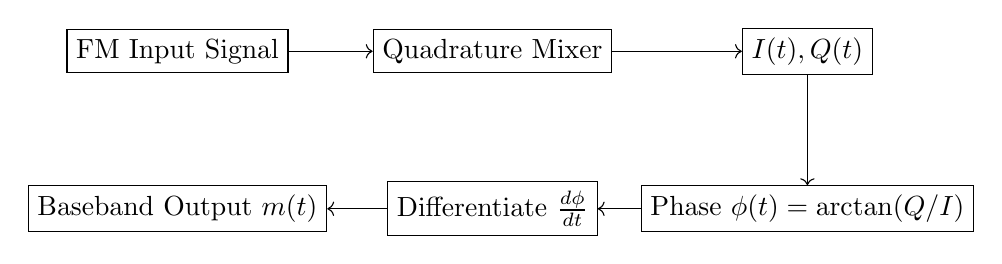
\begin{tikzpicture}[node distance=2cm,auto]
    % Nodes
    \node (in) [draw, rectangle] {FM Input Signal};
    \node (mix) [draw, rectangle, right of=in, node distance=4cm] {Quadrature Mixer};
    \node (iq) [draw, rectangle, right of=mix, node distance=4cm] {$I(t), Q(t)$};
    \node (phase) [draw, rectangle, below of=iq, node distance=2cm] {Phase $\phi(t) = \arctan(Q/I)$};
    \node (diff) [draw, rectangle, left of=phase, node distance=4cm] {Differentiate $\frac{d\phi}{dt}$};
    \node (out) [draw, rectangle, left of=diff, node distance=4cm] {Baseband Output $m(t)$};

    % Connections
    \draw[->] (in) -- (mix);
    \draw[->] (mix) -- (iq);
    \draw[->] (iq) -- (phase);
    \draw[->] (phase) -- (diff);
    \draw[->] (diff) -- (out);
\end{tikzpicture}
\end{center}

\section*{Relay Feedback 自動整定(Åström--Hägglund)}

\subsection*{關鍵公式}
理想繼電器輸出幅度為 $\pm h$,若閉迴路產生穩定極限循環,輸出正弦近似幅度為 $a$、週期為 $P_u=2\pi/\omega_u$,則
\[
N(a)=\frac{4h}{\pi a},\qquad
G(j\omega_u)\,N(a)=-1
\]
由此可得臨界增益
\[
K_u=\frac{4h}{\pi a}.
\]

\subsection*{控制框圖}
\begin{center}
\begin{tikzpicture}[
  block/.style={draw,rectangle,minimum height=10mm,minimum width=18mm,align=center},
  sumsym/.style={draw,circle,inner sep=0pt,minimum size=6mm}, % 這行是定義 sumsmy 樣式
  >={Stealth}
]
% Nodes
\node[block] (ref) {參考 $r(t)$};
\node[sumsym, right=12mm of ref] (adder) {$\sum$};
\node[block, right=12mm of adder] (relay) {繼電器\\$\pm h$};
\node[block, right=12mm of relay] (plant) {被控對象\\$G(s)$};
\node[block, right=12mm of plant] (meas) {輸出 $y(t)$};

% Connections
\draw[->] (ref) -- (adder);
\draw[->] (adder) -- node[above] {$e(t)$} (relay);
\draw[->] (relay) -- node[above] {$u(t)$} (plant);
\draw[->] (plant) -- (meas);
\draw[->] (meas.south) |- ++(0,-12mm) -| node[pos=0.75,below] {$-$} (adder.south);

\end{tikzpicture}
\end{center}

\subsection*{說明}
\begin{itemize}
  \item 將原控制器暫時以繼電器取代,閉迴路自然激發極限循環。
  \item 量測輸出振幅 $a$ 與週期 $P_u$,由 $K_u=\tfrac{4h}{\pi a}$ 推得臨界增益,再套用 Ziegler--Nichols 或其他整定規則得到 PID 參數。
\end{itemize}
================================================================
\section{The Role of $T/4$ Delay and $\pi/4$ Phase Bias}

\subsection{Phase Difference Analysis}

Consider a narrowband signal with a slowly varying phase:
\begin{equation}
s(t)=A\cos\bigl(\omega_c t+\phi(t)\bigr).
\end{equation}

The signal is delayed by a quarter of the carrier period,
\begin{equation}
\tau=\frac{T}{4}=\frac{\pi}{2\omega_c},
\end{equation}
resulting in
\begin{equation}
s(t-\tau)
= A\cos\!\left(\omega_c t-\frac{\pi}{2}+\phi(t-\tau)\right).
\end{equation}

To set the operating point at $\pi/4$, an additional fixed phase bias of $\pi/4$ is applied to the delayed path. The biased signal becomes
\begin{equation}
s_b(t)
= A\cos\!\left(\omega_c t-\frac{\pi}{4}+\phi(t-\tau)\right).
\end{equation}

\subsection{Multiplier Output}

The product of the original and biased delayed signals is
\begin{align}
s(t)\,s_b(t)
&= \frac{A^2}{2}
\Bigl[
\cos\!\left(2\omega_c t-\frac{\pi}{4}
+\phi(t)+\phi(t-\tau)\right)
\nonumber\\
&\quad
+\cos\!\left(\frac{\pi}{4}
-\bigl[\phi(t)-\phi(t-\tau)\bigr]\right)
\Bigr].
\end{align}

\subsection{Low-Pass Filtered Output}

After low-pass filtering, the high-frequency component is removed, leaving
\begin{equation}
\text{Output}
\propto
\cos\!\left(\frac{\pi}{4}-\Delta\phi(t)\right),
\end{equation}
where
\begin{equation}
\Delta\phi(t)=\phi(t)-\phi(t-\tau).
\end{equation}

\section{Why Choose $T/4$ and a $\pi/4$ Operating Point}

\subsection{Optimal Sensitivity}

The $T/4$ delay introduces a $\pi/2$ carrier phase shift, ensuring quadrature between the two signal paths. By applying an additional $\pi/4$ phase bias, the detector operates at a point of high linearity and sensitivity, providing an efficient phase-to-voltage conversion.

\subsection{Small-Signal Approximation}

For small phase variations $\Delta\phi$, the output can be approximated by
\begin{equation}
\cos\!\left(\frac{\pi}{4}-\Delta\phi\right)
\approx
\cos\!\left(\frac{\pi}{4}\right)
+\sin\!\left(\frac{\pi}{4}\right)\Delta\phi
=
\frac{\sqrt{2}}{2}
+\frac{\sqrt{2}}{2}\,\Delta\phi.
\end{equation}

Thus, around the $\pi/4$ operating point, the detector output varies linearly with the phase difference.

\subsection{Frequency Detection}

The instantaneous frequency deviation can be approximated as
\begin{equation}
\Delta\omega(t)
=\frac{d\phi(t)}{dt}
\approx
\frac{\phi(t)-\phi(t-\tau)}{\tau},
\end{equation}
with
\begin{equation}
\tau=\frac{T}{4}=\frac{\pi}{2\omega_c}.
\end{equation}
\section{Advantages of the $T/4$ Delay with $\pi/4$ Phase Bias Detector}

\subsection{Maximum Phase Sensitivity}

The use of a $T/4$ delay introduces a $\pi/2$ carrier phase shift, ensuring quadrature between the two signal paths. When combined with a $\pi/4$ phase bias, the detector operates at a point where the slope of the output with respect to the phase difference is maximized.

Specifically, the detector output is given by
\begin{equation}
\text{Output} \propto \cos\!\left(\frac{\pi}{4}-\Delta\phi\right),
\end{equation}
whose derivative with respect to $\Delta\phi$ is
\begin{equation}
\frac{d}{d(\Delta\phi)}
\cos\!\left(\frac{\pi}{4}-\Delta\phi\right)
=
\sin\!\left(\frac{\pi}{4}-\Delta\phi\right).
\end{equation}

At the operating point $\Delta\phi=0$, the slope becomes
\begin{equation}
\left.\frac{d(\text{Output})}{d(\Delta\phi)}\right|_{\Delta\phi=0}
=
\sin\!\left(\frac{\pi}{4}\right)
=
\frac{\sqrt{2}}{2},
\end{equation}
which represents a high and stable phase-to-voltage conversion gain.

---

\subsection{Improved Linearity for Small Phase Variations}

For small phase differences, the output can be linearized as
\begin{equation}
\cos\!\left(\frac{\pi}{4}-\Delta\phi\right)
\approx
\frac{\sqrt{2}}{2}
+
\frac{\sqrt{2}}{2}\Delta\phi.
\end{equation}

This approximation shows that the detector output consists of a constant bias term and a linear term proportional to the phase difference. Compared to detectors operating at $\Delta\phi=0$ or $\Delta\phi=\pi/2$, the $\pi/4$ operating point provides a wider linear region, making it well suited for small-signal phase and frequency detection.

---

\subsection{Reduced Sensitivity to Amplitude Fluctuations}

Because the two signal paths are orthogonal due to the $T/4$ delay, the low-pass filtered output primarily depends on the phase difference rather than the absolute signal amplitude. Slow amplitude variations affect both paths similarly and are largely canceled by the multiplication and filtering process.

As a result, the detector exhibits improved robustness against:
\begin{itemize}
\item amplitude modulation,
\item fading-induced gain variations,
\item front-end gain mismatch.
\end{itemize}

This property is particularly beneficial in practical sensing and communication systems where amplitude stability cannot be guaranteed.

---

\subsection{Enhanced Noise Performance}

The multiplication of the signal with a quadrature-delayed replica effectively performs coherent detection, which improves the signal-to-noise ratio (SNR) of the phase estimate. Furthermore, the low-pass filter suppresses high-frequency noise components around $2\omega_c$, leaving only the slowly varying phase-related term.

Operating at the $\pi/4$ bias point avoids the flat regions of the cosine response, where noise-induced phase fluctuations would produce minimal output variation. This results in improved phase resolution under noisy conditions.

---

\subsection{Suitability for Frequency Detection}

The phase difference obtained from the $T/4$ delay approximates the phase derivative:
\begin{equation}
\Delta\phi(t) \approx \tau \frac{d\phi(t)}{dt},
\end{equation}
which leads directly to an estimate of the instantaneous frequency deviation:
\begin{equation}
\Delta\omega(t)
\approx
\frac{\phi(t)-\phi(t-\tau)}{\tau}.
\end{equation}

Thus, the proposed structure naturally supports frequency discrimination without requiring explicit differentiation, making it attractive for frequency tracking and Doppler sensing applications.

---

\subsection{Implementation Efficiency}

The proposed detector relies only on:
\begin{itemize}
\item a fixed delay of $T/4$,
\item a constant phase bias,
\item a single multiplier,
\item and a low-pass filter.
\end{itemize}

No trigonometric operations or arctangent computations are required, which significantly reduces implementation complexity. This makes the structure well suited for real-time realization in digital signal processors (DSPs), field-programmable gate arrays (FPGAs), and software-in-the-loop (SIL) simulation frameworks.

---

\subsection{Summary of Advantages}

In summary, the $T/4$ delay with a $\pi/4$ phase bias offers:
\begin{itemize}
\item high phase sensitivity,
\item wide linear operating range,
\item robustness to amplitude fluctuations,
\item improved noise performance,
\item direct frequency discrimination capability,
\item and low implementation complexity.
\end{itemize}

These advantages make the proposed detector particularly suitable for phase- and frequency-based sensing and communication systems.

\section{Comparison with Arctangent-Based Phase Estimation}

Phase estimation can also be achieved using arctangent-based methods, which explicitly compute the phase from in-phase and quadrature components. This section compares the proposed $T/4$ delay with $\pi/4$ phase bias detector to conventional arctangent-based phase estimation in terms of sensitivity, linearity, noise robustness, and implementation complexity.

\subsection{Principle of Arctangent-Based Phase Estimation}

In arctangent-based phase estimation, the received signal is first converted into its in-phase and quadrature components:
\begin{equation}
I(t) = A\cos\phi(t), \quad Q(t) = A\sin\phi(t).
\end{equation}

The instantaneous phase is then obtained as
\begin{equation}
\hat{\phi}(t) = \tan^{-1}\!\left(\frac{Q(t)}{I(t)}\right).
\end{equation}

While this approach provides a direct phase estimate, it requires precise quadrature generation, division, and arctangent operations, which increase computational complexity and sensitivity to noise and amplitude imbalance.

---

\subsection{Sensitivity and Linearity}

The proposed detector produces a low-pass output of the form
\begin{equation}
\text{Output} \propto \cos\!\left(\frac{\pi}{4}-\Delta\phi\right),
\end{equation}
which can be linearized for small phase variations as
\begin{equation}
\text{Output} \approx \frac{\sqrt{2}}{2} + \frac{\sqrt{2}}{2}\Delta\phi.
\end{equation}

In contrast, the arctangent method exhibits a nonlinear response to noise due to the ratio $Q/I$, particularly when $I$ is small. The proposed detector avoids explicit division and maintains a well-defined linear operating region around the $\pi/4$ bias point, resulting in improved small-signal sensitivity.

---

\subsection{Noise Robustness}

In arctangent-based estimation, noise affects both $I$ and $Q$ components, and the nonlinear $\tan^{-1}(\cdot)$ operation can significantly amplify noise, especially near quadrant boundaries. Additionally, phase unwrapping is often required to maintain continuity.

The proposed detector relies on multiplication and low-pass filtering, which naturally suppress high-frequency noise components. By operating away from the extrema of the cosine response, the $\pi/4$ bias point ensures that noise-induced phase fluctuations translate into proportional output variations, enhancing robustness in low-SNR conditions.

---

\subsection{Amplitude Sensitivity}

Arctangent-based methods assume accurate amplitude matching between the $I$ and $Q$ channels. Any gain mismatch or amplitude fading can introduce phase estimation errors.

In contrast, the $T/4$ delay-based detector exhibits reduced sensitivity to amplitude variations because the two signal paths originate from the same signal and differ only by delay and phase bias. Common-mode amplitude fluctuations therefore largely cancel out, making the detector more robust to gain variations and fading.

---

\subsection{Computational and Implementation Complexity}

Arctangent-based phase estimation requires:
\begin{itemize}
\item precise quadrature signal generation,
\item division operations,
\item arctangent computation,
\item phase unwrapping logic.
\end{itemize}

These operations are computationally expensive and challenging to implement efficiently in fixed-point hardware.

The proposed detector, by contrast, requires only:
\begin{itemize}
\item a fixed $T/4$ delay,
\item a constant phase bias,
\item a single multiplier,
\item and a low-pass filter.
\end{itemize}

No transcendental functions are required, making the detector highly suitable for real-time implementation in DSPs, FPGAs, and software-in-the-loop (SIL) environments.

---

\subsection{Summary of Comparison}

Table~\ref{tab:comparison_phase_detectors} summarizes the key differences between the proposed detector and arctangent-based phase estimation.

\begin{table}[h]
\centering
\caption{Comparison of Phase Estimation Methods}
\label{tab:comparison_phase_detectors}
\begin{tabular}{lcc}
\hline
\textbf{Aspect} & \textbf{Proposed Method} & \textbf{Arctangent-Based} \\
\hline
Phase sensitivity & High (linear near $\pi/4$) & High but nonlinear \\
Noise robustness & High & Moderate \\
Amplitude robustness & High & Sensitive to imbalance \\
Computational complexity & Low & High \\
Hardware suitability & Excellent & Limited \\
Phase unwrapping required & No & Yes \\
\hline
\end{tabular}
\end{table}

Overall, the proposed $T/4$ delay with $\pi/4$ phase bias detector provides a favorable trade-off between sensitivity, robustness, and implementation efficiency, making it particularly attractive for practical phase- and frequency-based sensing systems.


\section{Limitation of the Sensing Range in SIL Radar}

In a software-in-the-loop (SIL) radar, the Doppler-induced phase shift of the received echo is actively canceled by introducing a tunable delay in the received signal path. By adjusting this delay, the SIL radar effectively eliminates the apparent phase variation of the echo, making the radar perceive a stationary target. This process is conceptually equivalent to electronically moving the radar in synchrony with the target motion. As a result, the target displacement can be directly extracted from the applied delay required to cancel the Doppler phase shift.

Although this approach removes the conventional $2\pi$ phase ambiguity, experimental results indicate that the linear sensing range is limited to approximately 14 wavelengths when the total harmonic distortion (THD) is constrained below 2.3\%. This section explains the origin of this limitation from both a system-level and a mathematical perspective.

\subsection{General System-Level Explanation}

In principle, delay-based Doppler cancellation allows the sensing range to exceed the sub-wavelength limitation of conventional phase-based radar systems. However, in practical implementations, the tunable delay is neither continuous nor unbounded. Several non-ideal factors limit the achievable sensing range.

First, the dynamic range of the tunable delay is finite, as it is typically implemented using digital delay lines, buffers, or fractional-delay filters. Once the required compensation delay exceeds this range, further Doppler cancellation becomes infeasible.

Second, and more critically, the delay resolution is finite. The minimum achievable delay step introduces a residual phase error, which accumulates as the displacement amplitude increases. This accumulated phase error manifests as nonlinear distortion in the extracted displacement signal, leading to increased harmonic content.

Finally, the SIL radar operates as a closed-loop system. As the target displacement grows, the corresponding Doppler phase rate increases, placing higher demands on the loop bandwidth and stability. Finite loop bandwidth and processing latency introduce phase lag, further degrading the accuracy of phase cancellation and contributing to nonlinearity.

Consequently, the reported sensing range of 14 wavelengths corresponds to the maximum displacement over which the combined effects of delay quantization, loop dynamics, and noise still allow highly linear operation.

\subsection{Mathematical Analysis of the Limitation}

The Doppler-induced phase of the received echo due to a target displacement $x(t)$ is given by
\begin{equation}
\phi(t) = \frac{4\pi}{\lambda} x(t),
\end{equation}
where $\lambda$ denotes the carrier wavelength.

In the SIL radar, a tunable delay $d(t)$ is introduced to cancel this phase variation. The phase shift introduced by the delay is
\begin{equation}
\phi_d(t) = \omega_c d(t),
\end{equation}
where $\omega_c$ is the carrier angular frequency. Doppler cancellation is achieved by enforcing
\begin{equation}
\phi(t) - \phi_d(t) \approx 0,
\end{equation}
which yields
\begin{equation}
d(t) \approx \frac{4\pi}{\omega_c \lambda} x(t).
\end{equation}

Using $\omega_c = 2\pi c / \lambda$, the delay-to-displacement relationship simplifies to
\begin{equation}
\label{eq:delay_displacement}
\boxed{
d(t) \approx \frac{2}{c} x(t)
}
\end{equation}
indicating that the tunable delay is directly proportional to the physical displacement.

In practice, the implemented delay contains a quantization error:
\begin{equation}
d(t) = \hat{d}(t) + \varepsilon_d(t),
\end{equation}
which results in a residual phase error
\begin{equation}
\varepsilon_\phi(t)
= \omega_c \varepsilon_d(t)
= \frac{4\pi}{\lambda} \varepsilon_d(t).
\end{equation}

For a harmonic displacement
\begin{equation}
x(t) = A \sin(\Omega t),
\end{equation}
the residual phase error introduces nonlinear distortion components in the recovered displacement signal. The resulting total harmonic distortion can be approximated as
\begin{equation}
\text{THD} \propto
\left( \frac{4\pi A}{\lambda} \right)^n \varepsilon_d,
\quad n \geq 2.
\end{equation}

As the displacement amplitude $A$ increases, the required delay swing grows proportionally, amplifying the effect of delay quantization and loop-induced phase errors. Consequently, the nonlinear distortion increases rapidly with displacement amplitude.

\subsection{Discussion and Interpretation}

The experimentally observed sensing range of 14 wavelengths corresponds to the maximum displacement amplitude for which the accumulated phase error remains sufficiently small to maintain a total harmonic distortion below 2.3\%. This limit is therefore not a fundamental physical constraint, but rather an engineering limit imposed by the finite delay resolution, dynamic range, and loop stability of the SIL radar implementation.

\subsection{Summary}

In summary, while delay-based Doppler cancellation in SIL radar removes the traditional $2\pi$ phase ambiguity and enables wide-range displacement sensing, the achievable linear sensing range is ultimately constrained by practical implementation factors. In the reported system, these factors limit the highly linear sensing range to approximately 14 wavelengths, within which excellent linearity and low harmonic distortion are maintained.


\section{Negative Frequency Considerations in Mixing: Mechanical Waves versus Electromagnetic Waves}

\subsection{Concept of Negative Frequency}

Negative frequency is a mathematical concept that arises naturally when signals are represented using complex exponentials. A real-valued sinusoidal signal can be expressed as
\begin{equation}
\cos(\omega t)
=
\frac{1}{2}
\left(
e^{j\omega t}
+
e^{-j\omega t}
\right),
\end{equation}
where the terms $e^{j\omega t}$ and $e^{-j\omega t}$ correspond to positive and negative frequency components, respectively. Physically, negative frequency does not represent a wave propagating in the opposite spatial direction, but rather a phase rotation in the opposite temporal direction within the complex representation.

\subsection{Mechanical Waves and Real-Valued Signal Representation}

Mechanical waves such as acoustic signals are inherently real-valued. Let $x(t)\in\mathbb{R}$ denote a measured acoustic pressure waveform. Its Fourier transform satisfies the conjugate symmetry property
\begin{equation}
X(-f) = X^{*}(f),
\end{equation}
which implies that positive and negative frequency components always appear as symmetric pairs.

As a consequence, negative frequencies in mechanical waves cannot be independently manipulated or observed. They are intrinsically linked to their positive-frequency counterparts and therefore do not require explicit consideration in most acoustic signal processing applications.

\subsection{Effect of Mixing on Mechanical Waves}

Mixing is performed through multiplication in the time domain. For an acoustic signal mixed with a real-valued local oscillator,
\begin{equation}
y(t) = x(t)\cos(\omega_0 t),
\end{equation}
the resulting frequency components are shifted to
\begin{equation}
\pm(\omega \pm \omega_0),
\end{equation}
where both positive and negative frequencies are translated symmetrically. Since the spectrum remains conjugate symmetric, no image-frequency ambiguity arises that would require separate handling of negative frequencies.

Therefore, in conventional acoustic signal processing, the effect of negative frequencies during mixing is implicitly accounted for and does not necessitate special treatment.

\subsection{Contrast with Complex Baseband Processing in RF Systems}

In radio-frequency (RF) and radar systems, signals are often represented using complex baseband (IQ) notation. Complex mixing is performed using
\begin{equation}
y(t) = x(t)e^{-j\omega_0 t},
\end{equation}
which shifts the spectrum asymmetrically. In this case, positive- and negative-frequency components are no longer constrained to be symmetric, and negative frequencies correspond to physically meaningful opposite phase rotations.

As a result, careful consideration of negative frequencies is essential in RF and radar systems to avoid image-frequency interference and to preserve Doppler sign information.

\subsection{When Negative Frequencies Matter in Mechanical Wave Processing}

Negative frequency considerations become relevant in mechanical wave processing only when complex analytic representations are intentionally introduced. An analytic signal can be constructed as
\begin{equation}
x_a(t) = x(t) + j\mathcal{H}\{x(t)\},
\end{equation}
where $\mathcal{H}\{\cdot\}$ denotes the Hilbert transform. This representation suppresses negative-frequency components and enables complex mixing behavior analogous to RF systems.

Such representations are employed in advanced acoustic applications including direction-of-arrival estimation, Doppler-based acoustic sensing, and array signal processing.

\subsection{Summary}

In summary, mechanical waves such as acoustic signals inherently contain both positive and negative frequency components due to their real-valued nature. However, these components are mathematically coupled and do not require explicit treatment in conventional mixing operations. In contrast, RF and radar systems employing complex baseband processing must explicitly account for negative frequencies, as they carry physically meaningful information related to phase rotation and Doppler direction.

\end{document}